%!TEX root = ../Hardtung_BA_SoSe20.tex

\section{Planning Solutions}
\label{sec:planningSolutions}

This section will build on the discovered usability issues found during the initial evaluation process (see Section \ref{sec:evaluation}). On this basis, first solutions can be planned that fix the most impactful usability issues. Furthermore, new features can be developed that increase productivity (by automating processes and part of the workflow), while also fixing the current problems.


\subsection{Graphical User Interface related changes}

These changes include everything that is related to the graphical user interface that the user interacts with.

\subsubsection{Overall UI Changes}
Every feature area (e.g. grid options, scaling options, arrow/symbol inputs etc.) should be seperated through a \texttt{EtchedBorder} with its name as the title. Within these borders, elements should follow a consistent order. This is why this hierarchy is being set for the placement within these areas: \texttt{JRadioButton, JTextField, JButton, JCheckBox}.

Though additional \texttt{JLabels} can be used to explain or to give indicators what the elements do specifically. Whenever possible, icons should replace text and tooltips should be used to give further explanation. Explanatory \texttt{JLabels} should only be used when icons and tooltips are not enough.

Additionally to the more consistent placement of elements within the UI, their sizes should be standardized as well. \texttt{JTextFields} for example should only be large enough to encapsulate the largest possible entry. This means that the \texttt{height} should always be set to 25 pixels ( and the \texttt{width} depending on what is being entered (e.g. entering an angle between 0-360° will be shorter than entering the textual explanation of a folding step).
\newline
\textbf{Fixes: \#2.01; \#2.02; \#2.03; \#4.01; \#4.03}\\
\newline
%Later Change
At a later point a complete redesign and rework of the UI will have to be carried out, in order to facilitate the goal of a unified and obstructionless design. At the current stage of development though the focus is being set to increase the efficiency and speed of creating origami diagrams, as this is the main reason why the Origrammer exists.

\subsubsection{Arrows \& Symbols}
A large part of the Origrammer is made up of the different arrows and symbols that can be used in diagrams. So far, these objects were simple vector graphics that were being placed on the diagram as \texttt{ImageIcons} of \texttt{JLabels}. This approach did initially work, but brought restrictions and problems with it.

 As vector graphics do not have explicit width or height values, the library Batik\cite{batik}, which was being used to load the .svg files, presented wrong values to the \texttt{JLabel.setBounds(width, height)}-method. As a result of this limitation, the arrows \& symbols got partially cut off at the original bounds of the \texttt{JLabel} when rotating them. To fix this issue, a new, pre-rotated vector graphic was being loaded whenever an arrow or symbol got rotated. Though this in turn facilitated itself in a wrong, always square border around the arrows and symbols. Additionally, this made interactions with arrows and symbols far slower and unflexible.
 
 Another sideeffect was a change in scale when rotating a non square object. A \texttt{JLabel} tries to display the biggest possible object that can fit within the border bounds. As seen on Figure \ref{fig:unwantedScaling} the size of the arrow changes after rotating it by 45°.

\begin{figure*}[htbp]
	\centering
	\begin{subfigure}{0.3\textwidth}
		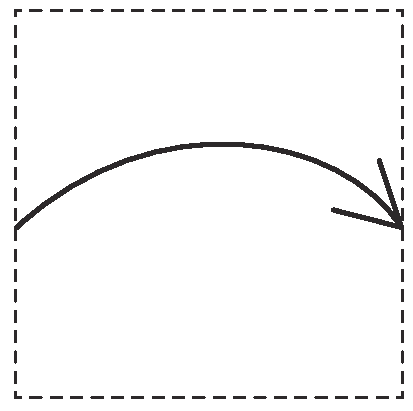
\includegraphics[width=\textwidth]{arrowLabelBorderStraight}
		\caption{Straight Arrow}
		\label{fig:arrowLabelBorderStraight}
	\end{subfigure}
	\begin{subfigure}{0.3\textwidth}
		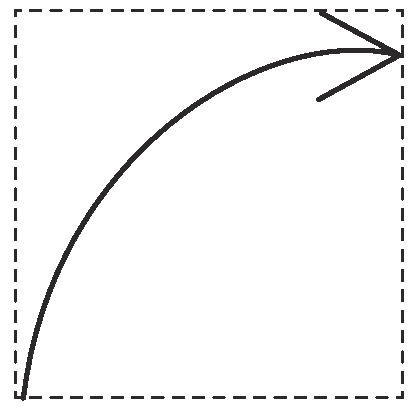
\includegraphics[width=\textwidth]{arrowLabelBorderAngled}
		\caption{Angled Arrow}
		\label{fig:arrowLabelBorderAngled}
	\end{subfigure}
	\caption{Unwanted Scaling when Rotating and the wrong, always square hitbox}
	\label{fig:unwantedScaling}
\end{figure*}

As a result of all these problems and limitations, the decision was made to completely rework how arrows \& symbols function in the Origrammer. The new approach was to rebuild all objects with simple \texttt{java.awt.Shape}-objects. This gave total control over rotations, scaling, and on-the-fly-editing of all arrows/symbols. Another advantage was the removed reliance on \texttt{JLabels} and associated with that, there were no longer issues with wrong hitboxes or different scaling while rotating. The only disadvantage was the work-intensive nature of remodeling all arrows and symbols with \texttt{Shape}-objects by hand.
\newline
\textbf{Fixes: \#1.02; \#7.05; \#7.06}

\subsubsection{Filling Tool}

The current limitations of the Filling Tool make it slow and cumbersome to use. The user has to manually input three vertices in order to create a triangle that shows the specified filling color. The limit of only three vertices per \texttt{OriFace}-object was originally introduced to give finer control for the user, as well as simplifying the development process for this feature.

But this decision went against the original goal of minimizing the time needed to create diagrams. As a result the Filling Tool has to be reworked, so that it can be used faster and with less user inputs.

\begin{figure}[htbp]
	\centering
	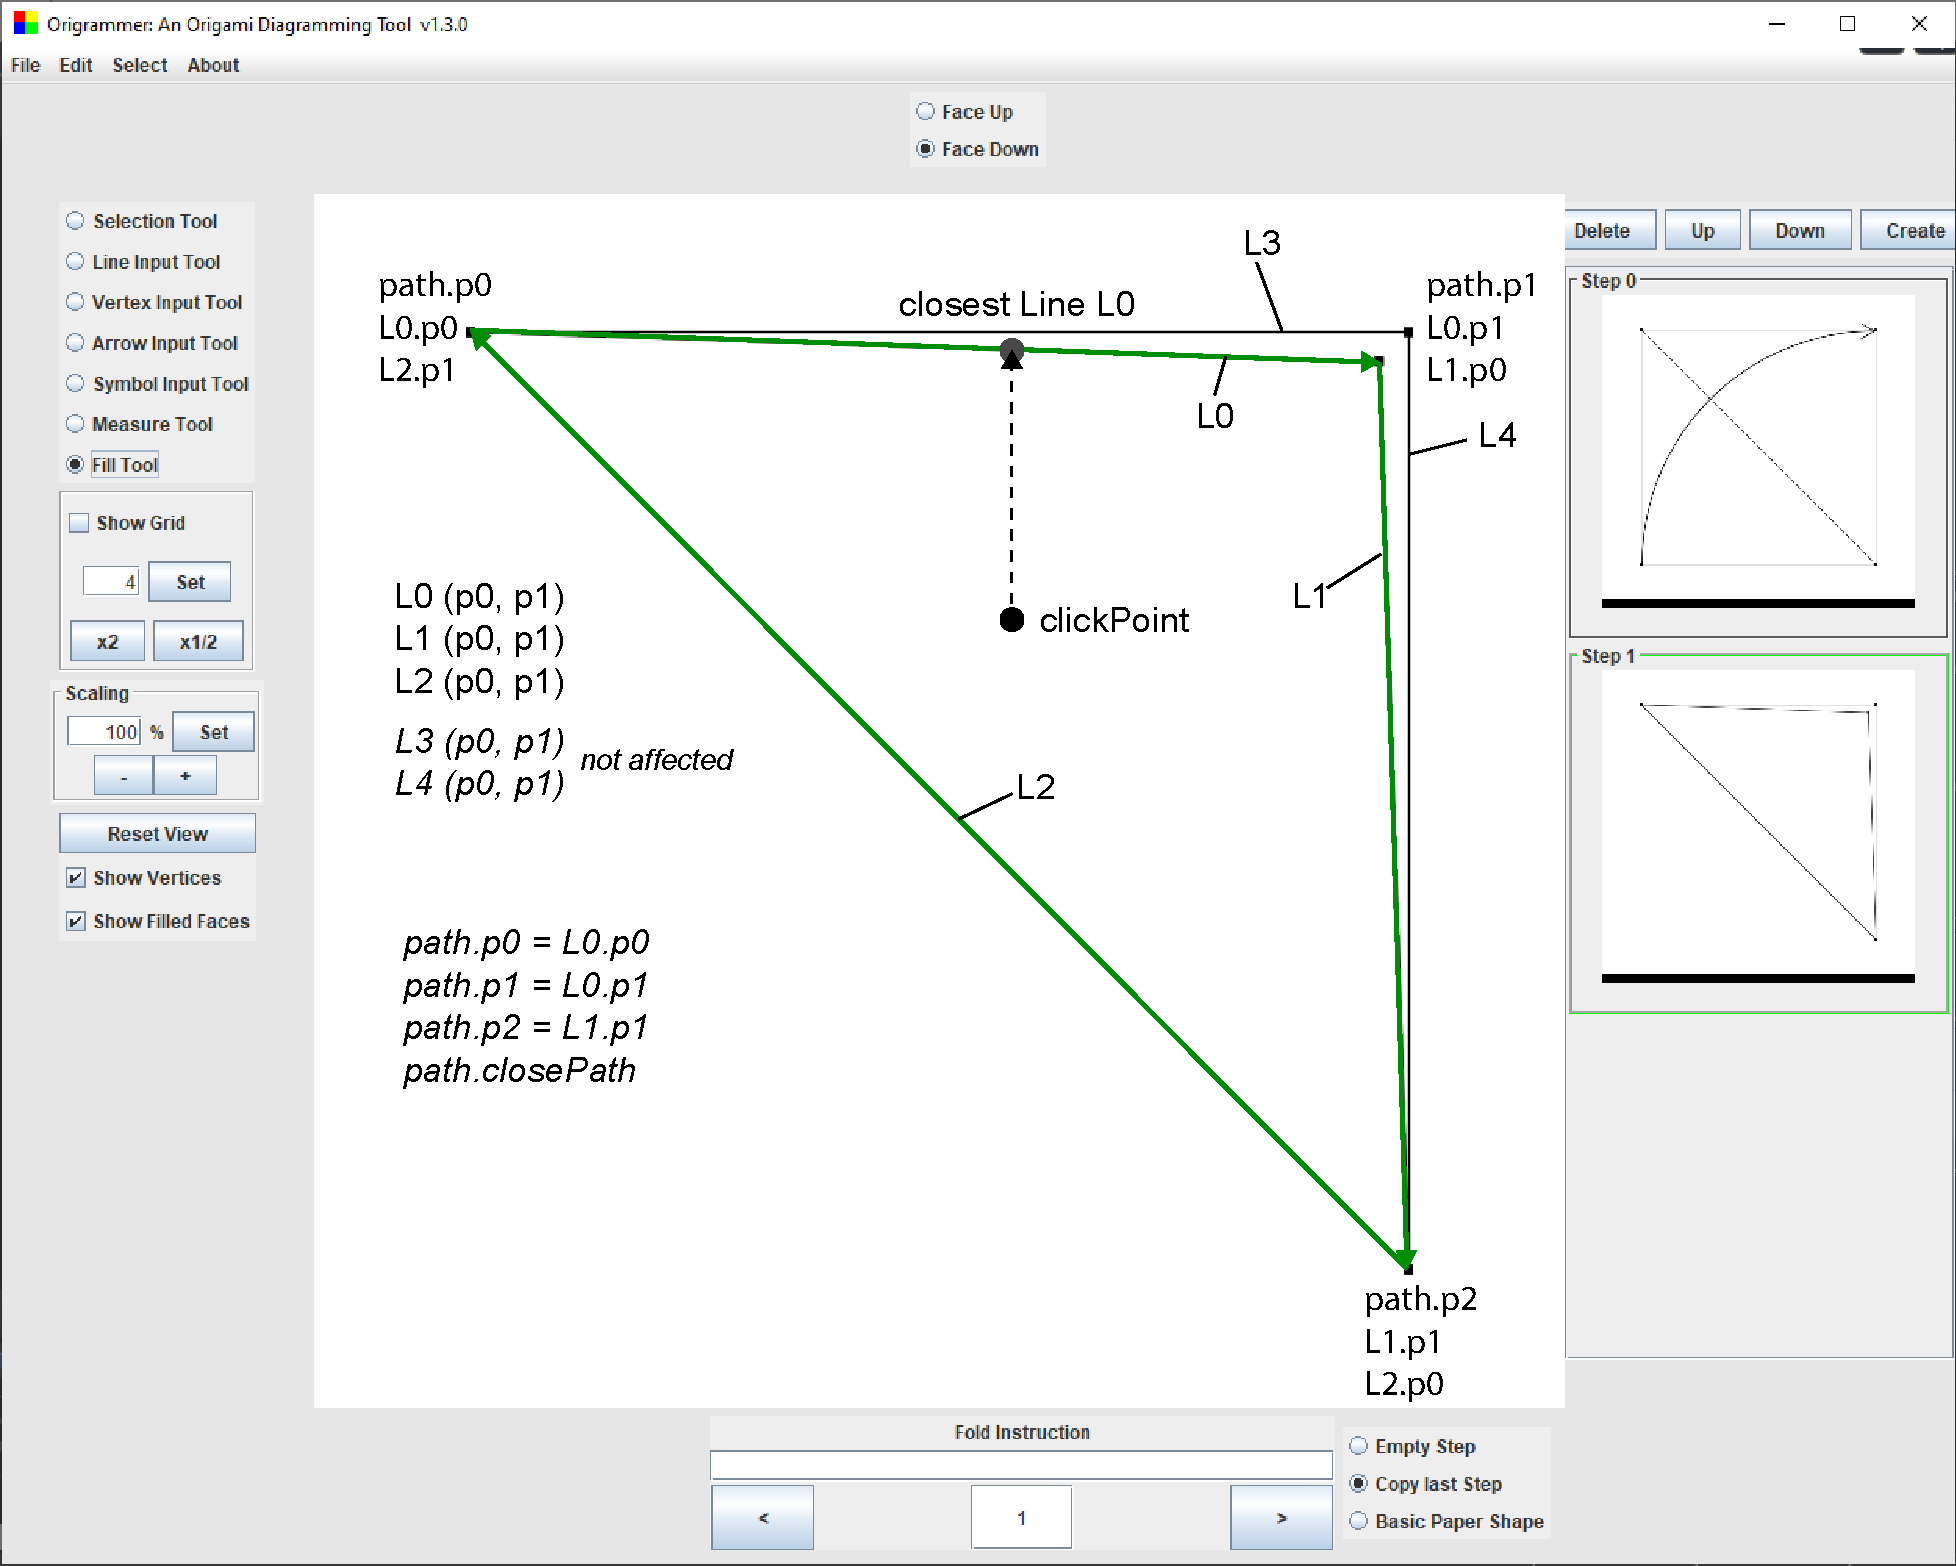
\includegraphics[width=0.9\textwidth]{fillingToolExample}
	\caption{Example on how the Filling Tool works after the rework}
	\label{fig:fillingToolExample}
\end{figure}
The new Filling Tool only requires one mouse click to fill an area with colour. When clicking in an area, the Origrammer first looks for the closest line to the \texttt{clickPoint}. Afterwards, both endpoints of the line are being checked for other touching or intersecting lines. The additional lines that were found have to be checked if they are visible from the original \texttt{clickPoint}, which would mean, that they are part of the enclosing lines. The endpoints of every new discovered line will be checked the same way, until a full enclosure of lines is established. Once this has happened, a \texttt{GeneralPath} is created that, goes through all points of the enclosing area. Lastly, the area of the \texttt{GeneralPath} can be filled with the specified colour.

%Finish explanations of how the Filling Tool works after the rework



\newpage
\subsubsection{Folding Presets}
In origami diagramming, there are eight widely established bases\cite{DesignSecrets} (p.53-64). When starting with these bases, one can fold a variety of different models. The bases in question are:

%\begin{itemize}
%\item Bird Base
%\item Kite Base
%\item Fish Base
%\item Frog Base
%\item Preliminary Fold
%\item Waterbomb Base
%\item Cupboard Base
%\item Windmill Base
% \end{itemize}
 
 \begin{figure}[htbp]
	\centering
	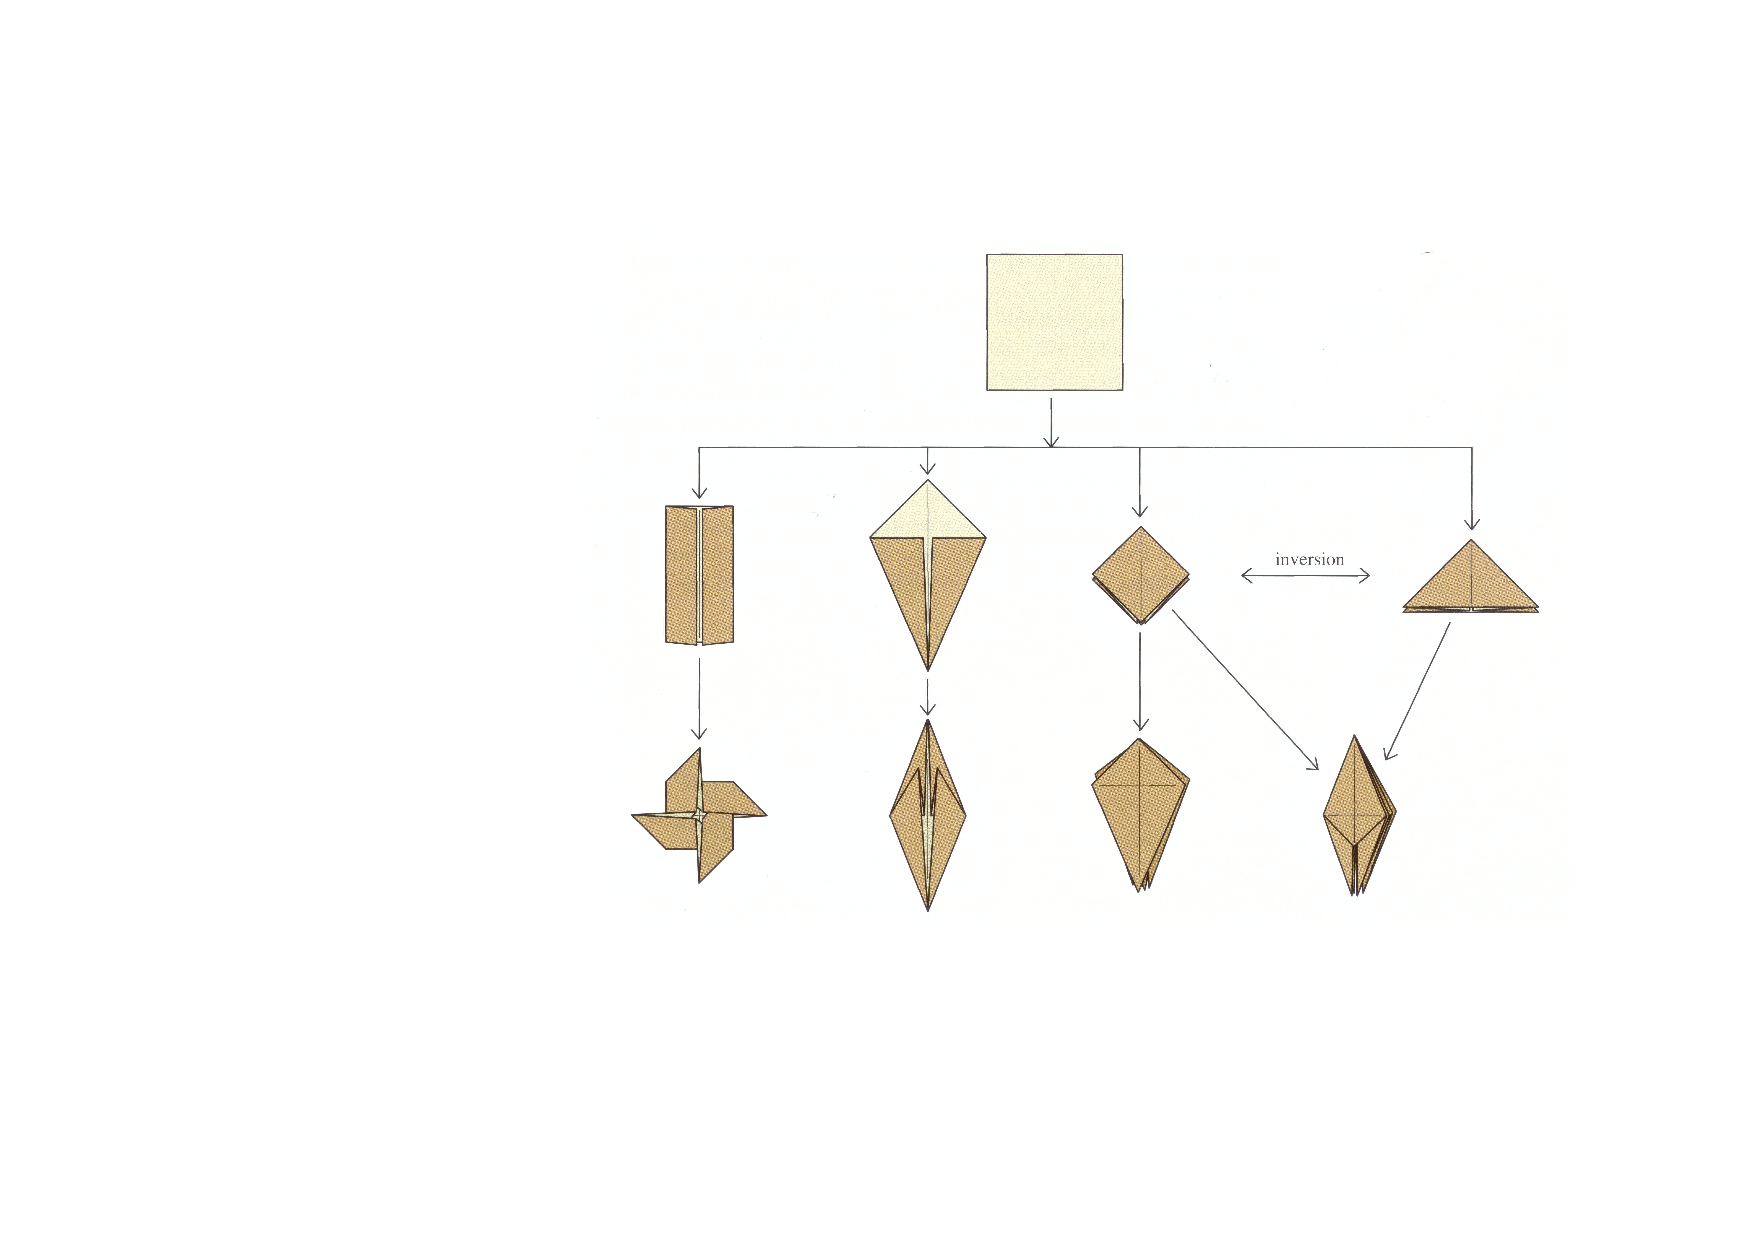
\includegraphics[width=0.8\textwidth]{BasesTree}
	\caption{Family Tree of the standard bases.\\
	Top to bottom and left to right:  Cupboard Base, Windmill Base, Kite Base, Fish Base, Preliminary Fold, Bird Base, Waterbomb Base, Frog Base - [Robert J. Lang 2011 \cite{BaseTree}]}
	\label{fig:basesTree}
\end{figure}

As these bases serve as the starting point for a wide array of models, it would be helpful to include them in the Origrammer. By giving the user the option to start a diagram with one of these bases, the overall diagramming process will be shortened by quite a bit. Not having to keep repeating the same beginning steps for different models will save time and can also show beginners of the program, how parts of the Origrammer look like or work.

Additionally to the origami bases, instructions on how to fold different grid sizes, should be included in the folding presets as well. Folding a 3x3, 5x5, or 7x7 grid from a square paper is not as straight forward and requires multiple folding steps to achieve. 

 \begin{figure}[htbp]
	\centering
	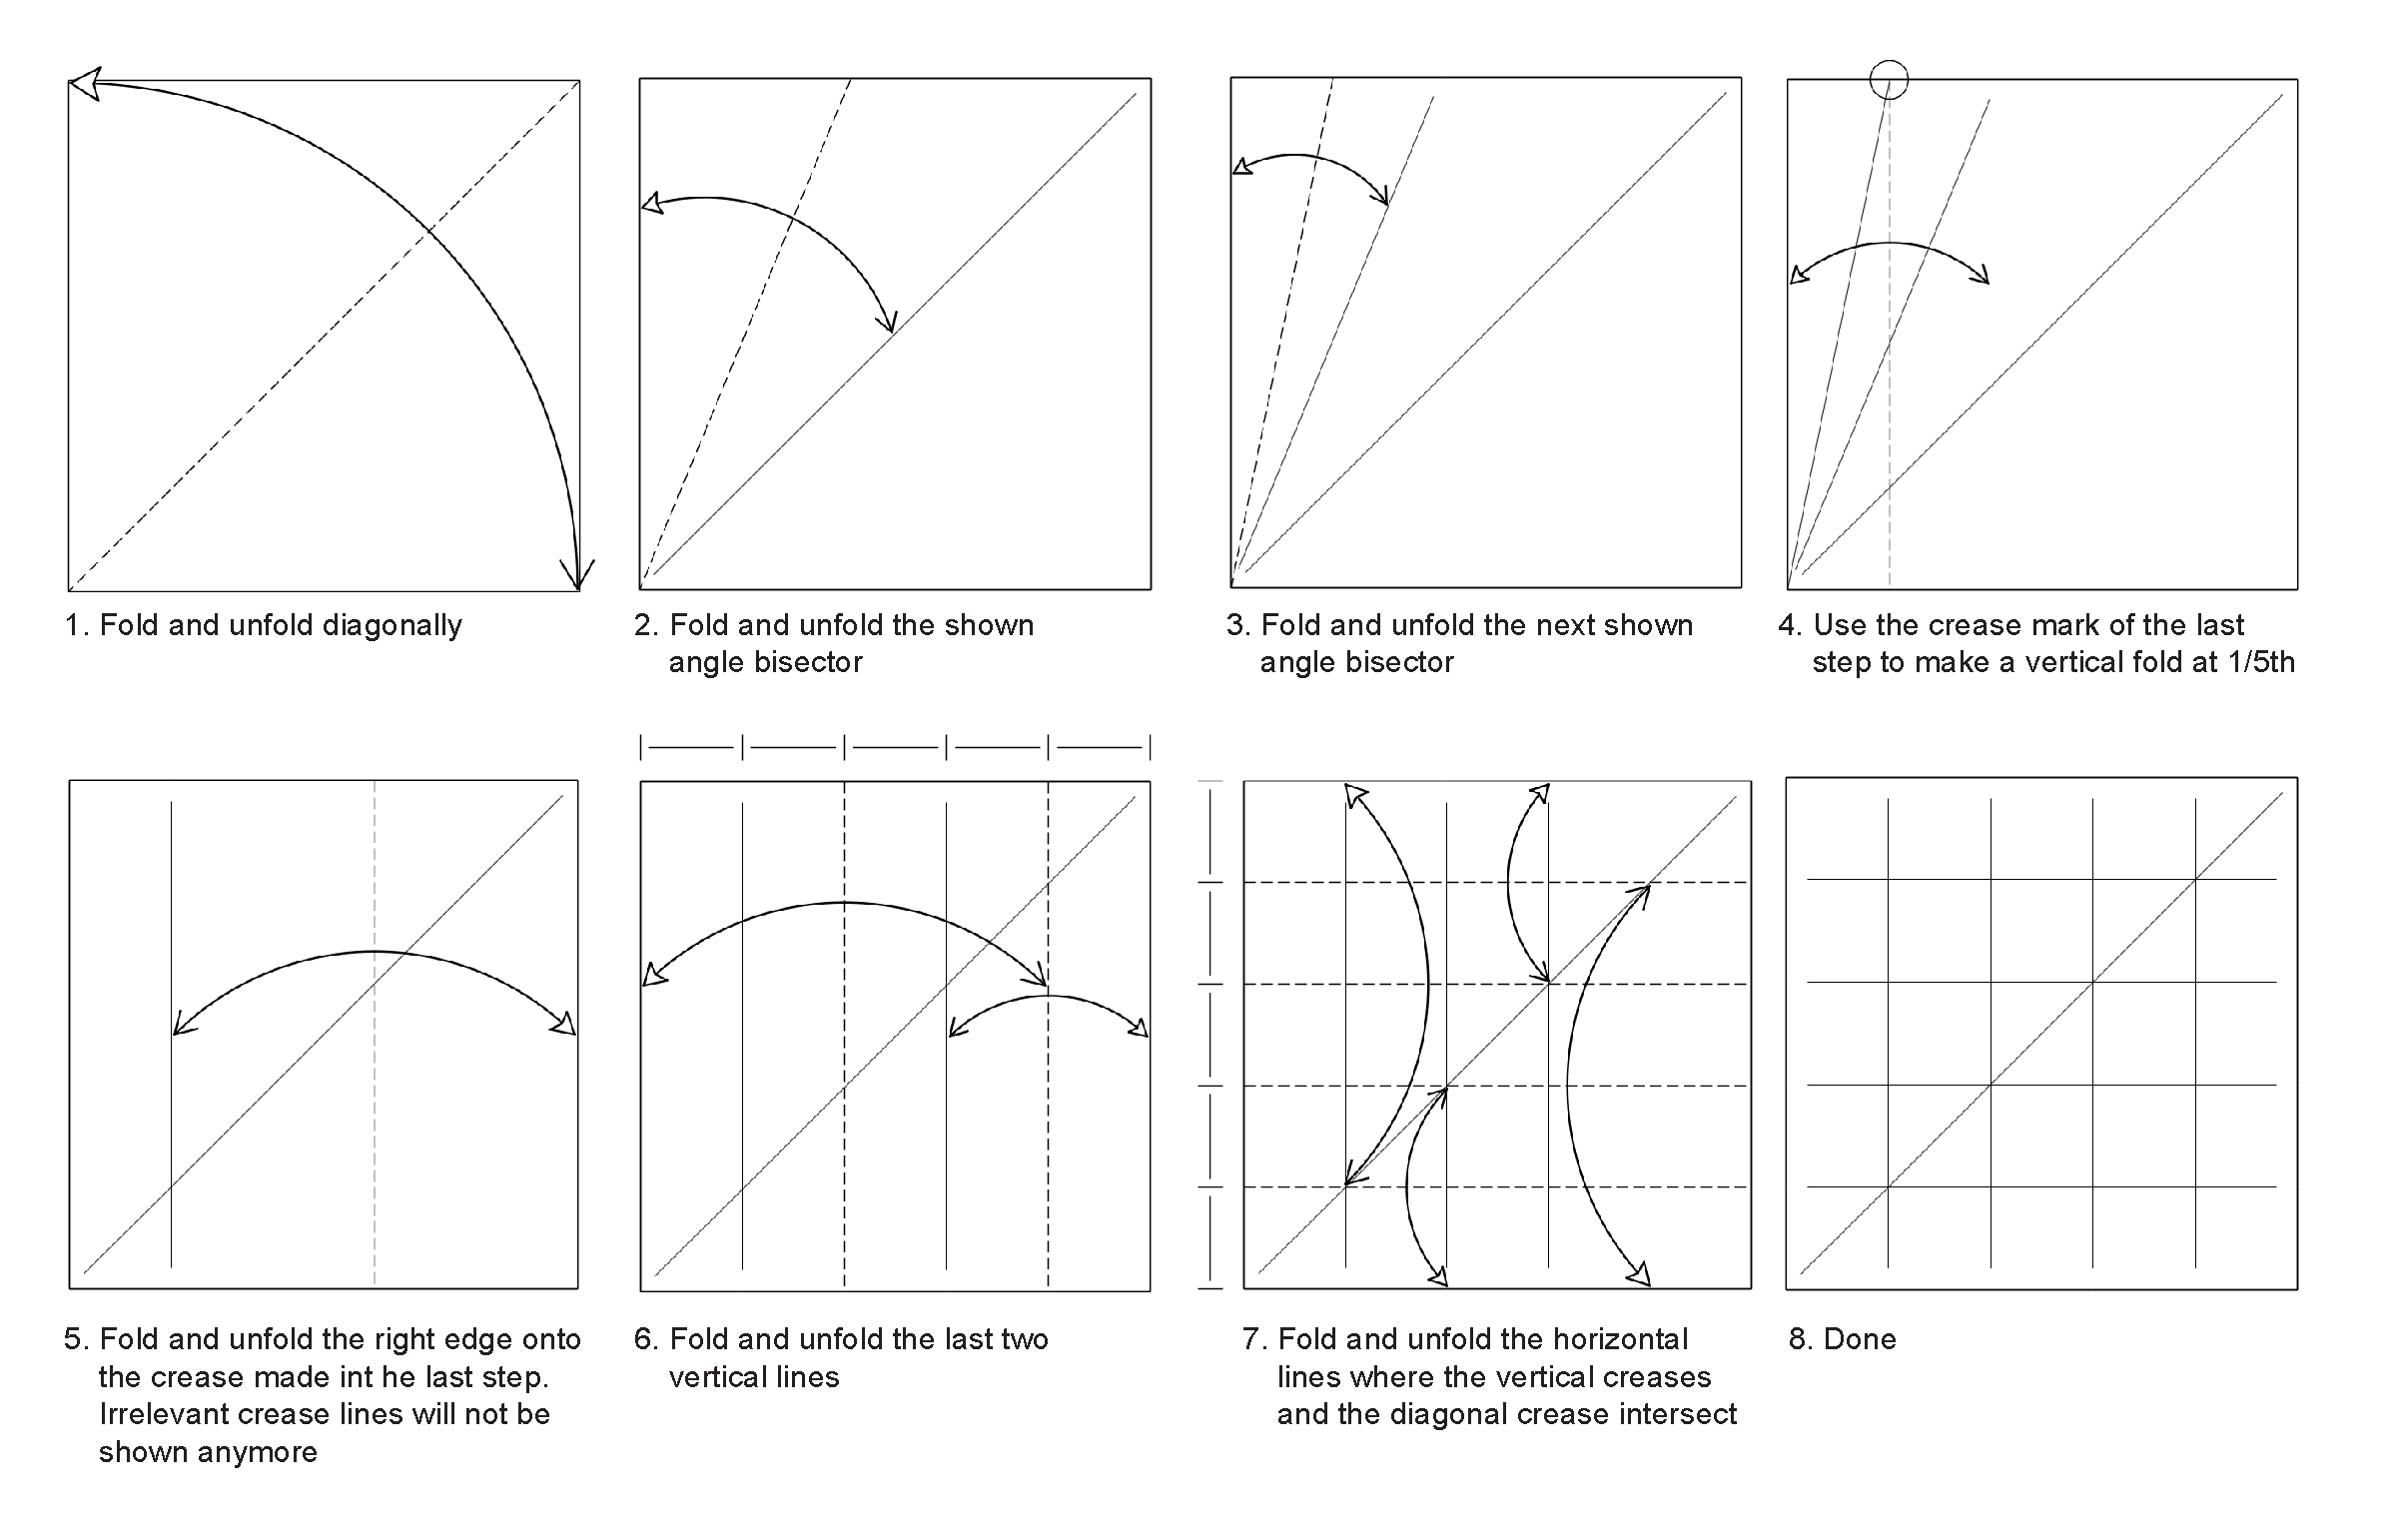
\includegraphics[width=\textwidth]{5x5-grid}
	\caption{Example diagram of a 5x5 grid made with the Origrammer}
	\label{fig:5x5-grid}
\end{figure}


\textbf{Fixes: \#7.09}

\subsubsection{Side Panel}

The text of the \texttt{JRadioButtons} at the tool bar should be replaced by self-explanatory icons in order to improve overall clarity. But the textual explanation of all the tools should still be present to help especially novizes. This can be done through tooltips that appear when hovering over the buttons.

\textbf{Fixes: \#2.01; \emph{\#2.03}}

\subsection{User Input related changes}

\subsection{New Origrammer features}

These new features should increase the productivity and efficiency of the Origrammer. The focus should be set on maximising the work that can be done in the shortest amount of time. This will be achieved by implementing features that either automate parts of the workflow, or that give new, faster possibilities of achieving the goal.

\subsubsection{Step Navigation \& Step Editing Options}

Currently, the Origrammer can create new diagram steps with three different options (\emph{Empty Step}, \emph{Copy last Step}, and \emph{Basic Paper Shape}). Furthermore the user can navigate through them with a \emph{Next-Step}-/ and a \emph{Previous-Step}-button. Though this approach brings limitation with it. Moving through the steps one by one hinders the overall usefulness and especially the speed of working with the Origrammer.

%delete and move and create in between
Deleting redundant steps can be quite important once the folding sequence goes through changes or simply when the user has made a mistake. In the same sense of offering solutions to user made mistakes, the Origrammer should make it possible to move steps to a different position within the diagram. Being able to create new steps in between existing ones can also be quite useful in negating user error.

%preview and make step active through clicking
An additional problem arises, once a diagram with a lot of steps (100+) is created. As the user currently only knows where he is in the folding sequence by the step number, this can lead to confusion. For example when folding an animal, there can be a different folding sequence, depending on what the artist decides to fold first (e.g. head first, the front or the hind legs, the tail, the abdomen, or the back). In order to continuously see where the user is within the diagram, there should be a small preview picture for all the steps within the step navigation. This will give the user an idea on what area a range of steps is working on. When clicking on one of the previews, the clicked step should made active and should be displayed on the Editing Panel.

As a result of the mentioned issues, the step navigation will be reworked to offer more functionality, visibility and ease of use. This will be accomplished by offering the following features in the rework:

\begin{itemize}
\item Small preview picture of a step
\item Click on preview picture to show the step in the Editing Panel
\item Show step number, the preview picture, as well as the folding description of the step in the navigation
\item Delete a selected step
\item Move a selected step to the front or the back
\item Create a new step between existing steps
\end{itemize}

\textbf{Fixes: \#1.03; \#3.02;   \#7.07}


\subsection{Virtual Folding of the Paper}
\label{sec:virtualFolding}

When creating diagrams with the Origrammer, the most time consuming activity is the placement of all required lines. All edges, current creases and existing creases have to be placed precicely, in order to allow the folder to closely follow the instructions simply by the visual cues. This large bottleneck in the diagramming process can only be eliminated by simulating the actual folding process virtually.

Being able to drag and drop a corner or edge of the paper to the desired position would reduce the work required by a large amount.

 \begin{figure}[htbp]
	\centering
	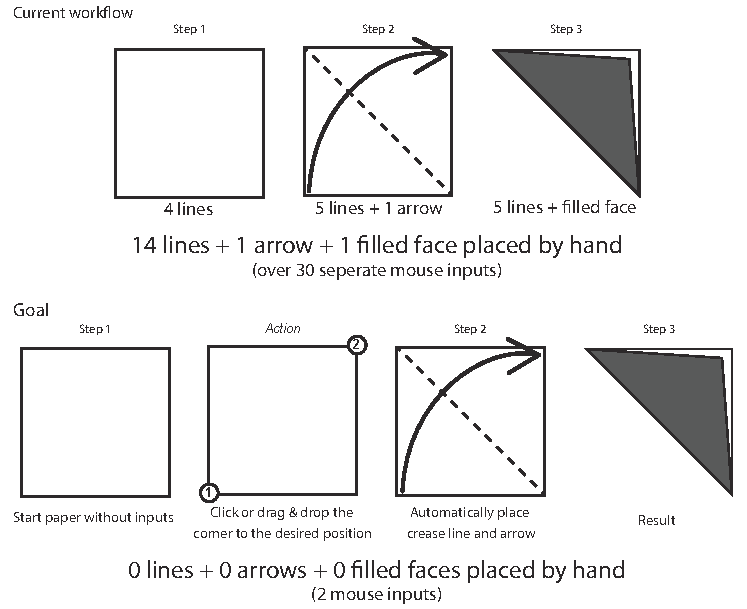
\includegraphics[width=\textwidth]{virtualFoldingGoal}
	\caption{Current workflow (top) \& Desired workflow (bottom)}
	\label{fig:virtualFoldingGoal}
\end{figure}

In order to implement this automated folding, several parts of the Origrammer have to be reworked.\\

\subsubsection*{Requirements}

The following aspects have to be kept track of in order to implement the system of virtual folding.

The paper lines have to be stored in a way, where their relations and connections to each other are stored and preserved. Then, as seen in Figure \ref{fig:virtualFoldingGoal}, the folding arrows have to be placed automatically when folding part of the paper. The folding line where the new crease is created should be created and placed automatically as well. This crease line might also have to go through multiple layers of paper, which will have to be checked against for each folding action. Lastly, the folded part of the paper has to actually change position and direction, and possibly show the differently colored side of the paper.\\

\subsubsection*{Current Status}

So far, every line got stored within a single \texttt{ArrayList<OriLine>} and was otherwise completely independent of the other lines. An additional \texttt{ArrayList<OriVertex>} was kept track of, in order to efficiently iterate through all vertices that can be used as an input point for new lines, arrows or symbols. All arrows and symbols got also stored within their respective \texttt{ArrayList<>} per folding step. Lastly, the folding steps themselves got stored within an \texttt{ArrayList<Step>} as well, which made saving the full diagram in a .xml-file simple and efficient.

This approach worked while there were no dependencies between the lines and vertices. But when folding virtually, several dependencies and other values have to be kept track of. These include among others the edge lines, existing creases, newly made creases (all with their specific line types), correct layering when rendering folded paper, correct colouring of different paper sides, and the rendering with slight distortions to show hidden layers/flaps (as on p.7 \emph{Distort the model to show all the layers} \cite{origrammer}).

\subsubsection*{Reworked System}

The new implementation works by splitting the actual paper model into \texttt{OriPolygons} that can be folded, split up, and rendered (see Listing \ref{oriPolygon}).

\begin{lstlisting}[label=oriPolygon,caption=OriPolygon]
OriPolygon {
        OriVertexList vertexList; 
        ArrayList<OriLine> lines;
        int height; /*height of the polygon for rendering order*/
}
\end{lstlisting}

Once the user inputs a new fold line, the Origrammer checks which \texttt{OriPolygons} are affected by the fold and subsequently splits them at the points where the folding line crosses the edges of a given polygon. The resulting line at the newly created crease is now a shared line between the two smaller, split up polygons. This is more closely visualized at Figure \ref{fig:reworkedPaperRepresentation}.
 \begin{figure}[htbp]
	\centering
	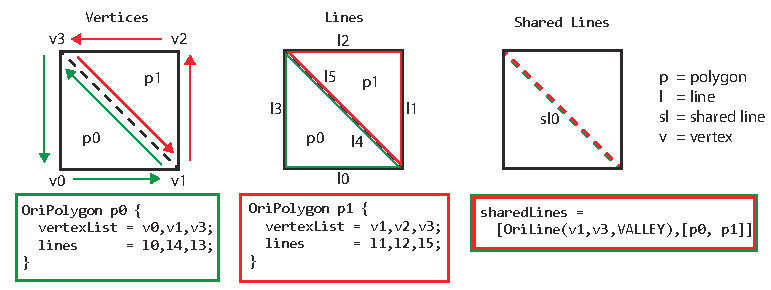
\includegraphics[width=\textwidth]{reworkedPaperRepresentation}
	\caption{Reworked Paper Representation through \texttt{OriPolygons} and \texttt{sharedLines}}
	\label{fig:reworkedPaperRepresentation}
\end{figure}

Every \texttt{OriPolygon} in turn consists of a \texttt{OriVertexList}, which contains all vertices of said polygon in a counter-clockwise order. Additionally, an \texttt{ArrayList<OriLine>} is required to keep track of the edge lines of the paper. As an \texttt{OriLine} also includes the line type, the lines within the \texttt{OriPolygon.lines}-list can have the type \texttt{EDGE} or \texttt{SHARED}.

For the case when a polygon is sharing a ling with another polygon, the \texttt{HashMap<OriLine, ArrayList<OriPolygon>> sharedLines} was added.

\begin{lstlisting}[label=paperModelImplementation,caption=New Implementation of Paper Model]
ArrayList<OriPolygon> polygons

HashMap<OriLine, <ArrayList<OriPolygon>> sharedLines
\end{lstlisting}

This \emph{shared lines}-list contains all the shared lines in combination of which polygons are sharing the given line. Additionally, the real line type is stored here, which is later used for rendering. If the \texttt{OriPolygons} would store the actual line type instead of the mockup type \texttt{SHARED}, then there would be no programmable connection between several \texttt{OriPolygons}. This would make folding lines that go through multiple polygons at the same time harder to calculate and progress from.\\

Alternatively, there could be a flag for each \texttt{OriLine} that would signalize if it also is a shared line. But then you would have to iterate through all \texttt{OriPolygons} and check every line in them when looking for the connected polygon of a given shared line. So even though the \texttt{HashMap} of shared lines has to be updated and kept track of at all times, it is still more flexible and efficient compared to the system of flagging an \texttt{OriLine} as a shared line.

\begin{lstlisting}[label=oriVertexList,caption={OriVertexList, OriVertex, and OriLine}]
OriVertexList {
        int n; /*vertex count*/
        OriVertex head;
}

OriVertex {
        Vector2d p; /*Vector2d(x, y)*/
        OriVertex prev;
        OriVertex next;
}

OriLine {
        OriVertex p0;
        OriVertex p1;
        int type; 
        /*NONE, EDGE, MOUNTAIN, VALLEY, XRAY, CREASE, 
        (SHARED), (DIAGONAL)*/
}
\end{lstlisting}

\newpage

 \begin{figure}[htbp]
	\centering
	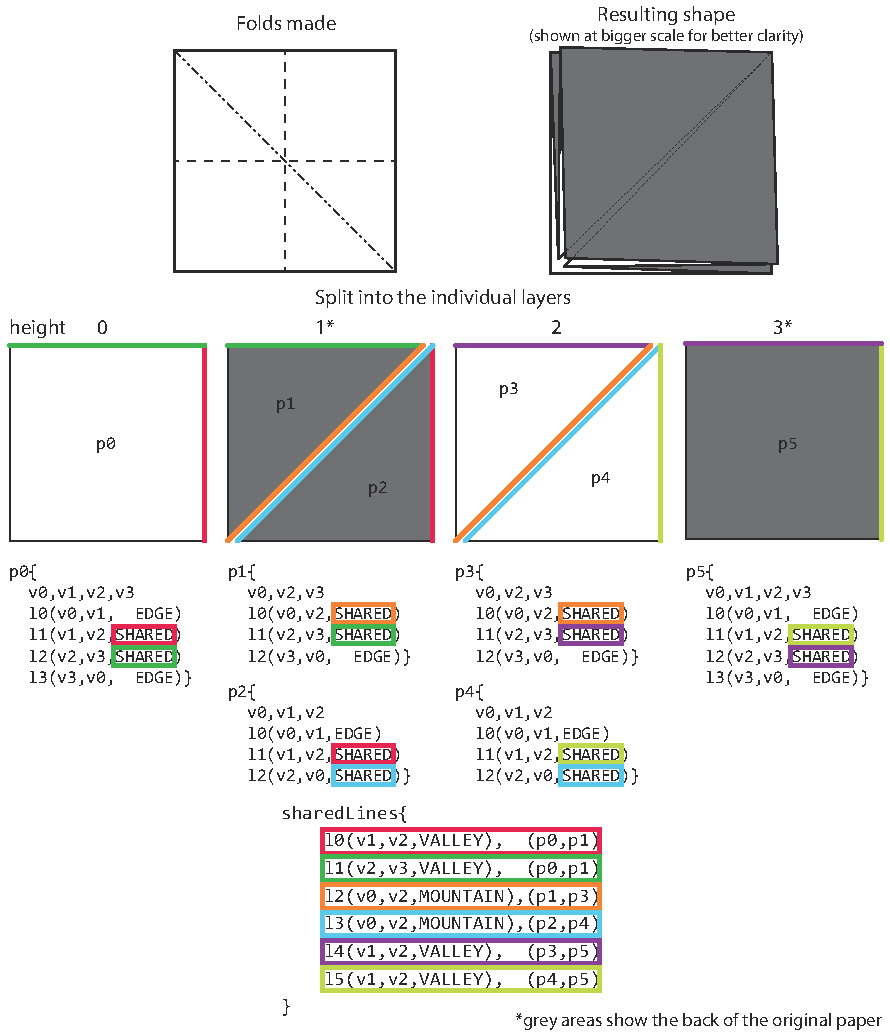
\includegraphics[width=\textwidth]{complexVirtualFolding}
	\caption{A more complex example of splitting polygons and multiple layers}
	\label{fig:complexVirtualFolding}
\end{figure}

The example in Figure \ref{fig:complexVirtualFolding} shows a slightly more complex example, on how the Origrammer splits the polygons and creates the correct shared lines. Additionally, in this case multiple layers of the paper have to be rendererd and kept track of. This height value is only preserved for each \texttt{OriPolygon} and is not used in the vertices, lines, or shared lines. It can be seen that for each shared line there can only be two \texttt{OriPolygon}s that share one edge. So when making a fold on one polygon and said fold crosses a shared line of this polygon, the Origrammer only has to search for the counterpart polygon, that shares the same line. This process can be seen in Figure \ref{fig:heightValuesWhenFolding}, where a fold through multiple layers is carried out. Internally, the Origrammer starts with a simple folding line on the top polygon that goes to its edges. If one or both endpoints of the folding line end in a shared line, it is clear that other polygons are also affected by this fold. Then one only has to iterate through the list of shared lines and find the connected polygon/s. Once the new \texttt{OriPolygon}/s have been found, the same process can then be repeated.


\begin{itemize}
\item Create the folding line on the top layer
\item Check both endpoints if they are ending in a shared line
\item Find the connected polygons on the sides that have a shared line
\item Repeat until on layer 0 or no other polygons are found

\end{itemize}



 \begin{figure}[htbp]
	\centering
	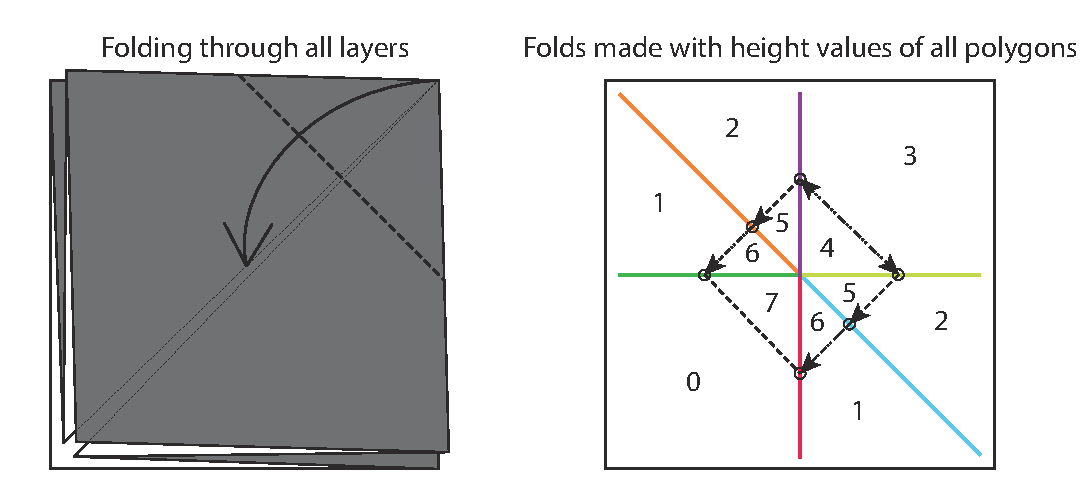
\includegraphics[width=\textwidth]{heightValuesWhenFolding}
	\caption{The process of folding through multiple layers and the updated height values}
	\label{fig:heightValuesWhenFolding}
\end{figure}



 \begin{figure}[htbp]
	\centering
	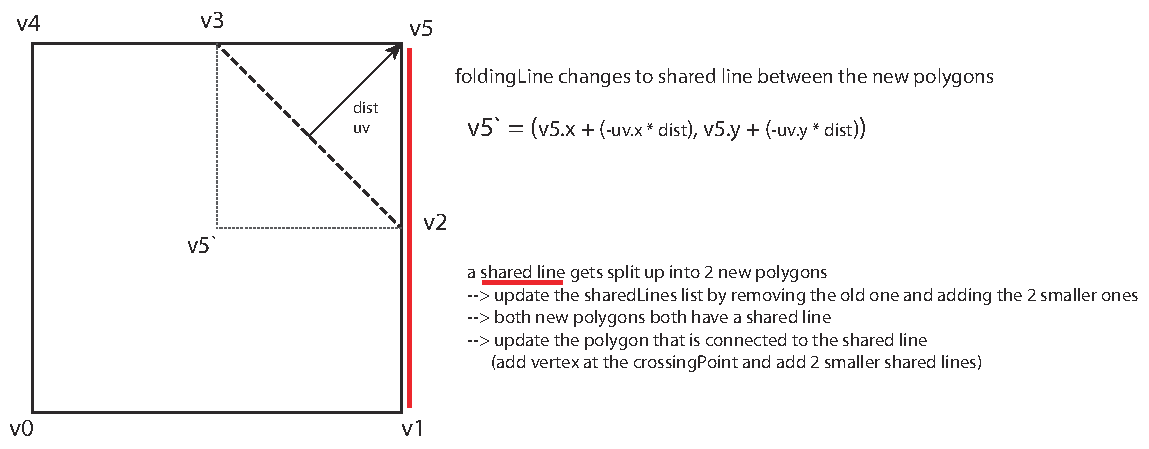
\includegraphics[width=\textwidth]{updatingVerticesWhenFolding}
	\caption{Process of updating the new vertex positions after folding and splitting existing shared lines}
	\label{fig:updatingVerticesWhenFolding}
\end{figure}
